\newpage
\section{Implementacja EMS-API}
Implementację możemy podzielić na dwa główne moduły - implementację aplikacji w Pythonie - EMS-API, która zostanie omówiona w tym rozdziale, oraz implementację interfejsu użytkownika w TypeScript, która będzie omówiona w kolejnym.

\subsection{Podział kodu}
Implementacja systemu EMS-API może zostać podzielona na implementację API, połączenia do Postgres oraz połączenia do Elasticsearch.

\textbf{Paczki:}
\begin{itemize}
    \item app - paczka z kodem implementującym API
    \item database - paczka z kodem implementującym podłączenie do bazy Postgres
    \item elastic\_utils - paczka z kodem implementującym podłączenie do Elasticsearch
    \item package\_utils - paczka z częściami wspólnymi np. implementacją logger'a
\end{itemize}


\subsection{Implementacja API}
\subsubsection{Podział kodu w API}
\begin{itemize}
    \item models - paczka z kodem reprezentującym modele. Modele są to definicje formatu danych przyjmowanych i zwracanych przez API
    \item routers - implementacja router'ów
    \item utils - paczka z częściami wspólnymi kodu
    \item main.py - główny plik API łączący wszystkie router'y
\end{itemize}
\subsubsection{Implementacja main.py}
API zostało zaimplementowane z pomocą biblioteki FastApi, która umożliwia wygodne definiowanie kolejnych endpoint'ów oraz podział logiczny kodu na kolejne pliki z zdefiniowanymi endpoint'ami. W głównym pliku znajduje się dodanie router'ów:
\begin{minted}{python}
    app = FastAPI()
    
    app.include_router(posts_router.router)
    app.include_router(security_router.router)
    app.include_router(estates_router.router)
    ...
\end{minted}
\subsubsection{Implementacja przykładowego router-a}
Każdy z routerów jest odpowiednio zdefiniowaną grupą end-pointów, w których możemy określić między innymi czy wymagane jest, aby użytkownik był zalogowany w momencie próby pozyskania danych z endpoint'u: poprzez użycie "dependencies". Poniżej przykład konfiguracji router'a z prefix-em requests do obsługi zgłoszeń:
\begin{minted}{python}
    router = APIRouter(
        prefix="/requests",
        tags=["requests"],
        responses={404: {"description": "Not found"}},
        dependencies=[Depends(get_current_active_user)]
    )
\end{minted}

W ramach danego router'a jesteśmy w stanie zdefiniować wiele endpoint'ów, w których definiujemy poza parametrami wejściowymi, w jakim formacie mają być zwrócone dane używając: response\_model. Poniżej przykład endpoint'u do odczytania konkretnego zgłoszenia: 
\begin{minted}{python}
    @router.get("/{request_id}", response_model=Optional[RequestInfo])
    async def get_request_( request_id: str,
                            current_user: Annotated[Users, 
                            Depends(get_current_active_user)],
                            db: Session = Depends(get_db)):
        return get_request(db, request_id, current_user.id)
\end{minted}
Jak można zauważyć, używany jest w nim response\_model: RequestInfo. Wszystkie takie modele zdefiniowane są w  folderze models.
\subsubsection{Implementacja przykładowego modelu}
Poniżej znajduje się implementacja przykładowego modelu, są to klasy, których reprezentacje są przekazywane do i z API.
\begin{minted}{python}
    from pydantic import BaseModel

    class RequestInput(BaseModel):
        title: str
        description: str
    
    class RequestInfo(RequestInput):
        id: str
        author_id: str | None
        title: str
        description: str
        department: str | None
        status: str
        start_time: datetime.datetime
        end_time: datetime.datetime | None
        assignee_id: str | None
        visibility: str
\end{minted}
\subsection{Implementacja połączenia z bazą Postgres}
Do obsługi bazy danych wykorzystany został ORM - SQLAlchemy, umożliwiający reprezentację relacji jako obiekty w kodzie.
\subsubsection{Podział kodu}
\begin{itemize}
    \item declarations - paczka ze zdefiniowanymi relacjami
    \item utils.py - plik z częściami wspólnymi kodu
\end{itemize}
\subsection{Implementacja użycia bazy Postgres}
W celu połączenia zdefiniowano url oraz tworzona jest sesja, która jest przekazywana do funkcji wykonujących operacje na bazie.
\begin{minted}{python}
    url = URL.create(
        drivername="postgresql+pg8000",
        username=POSTGRESQL_USERNAME,
        password=POSTGRESQL_PASSWORD,
        host=POSTGRESQL_HOST,
        port=POSTGRESQL_PORT,
        database=DATABASE_NAME
    )
    SessionLocal = sessionmaker(autocommit=False, autoflush=False,
                                bind=SqlEngine().engine)
\end{minted}
\subsubsection{Sposób reprezentacji relacji}
Każda relacja ma odwzorowanie w obiekcie. Relacje zaimplementowane zostały na podstawie modelu stworzonego w narzędziu dbdiagram:
\begin{figure}[H]
    \centering
    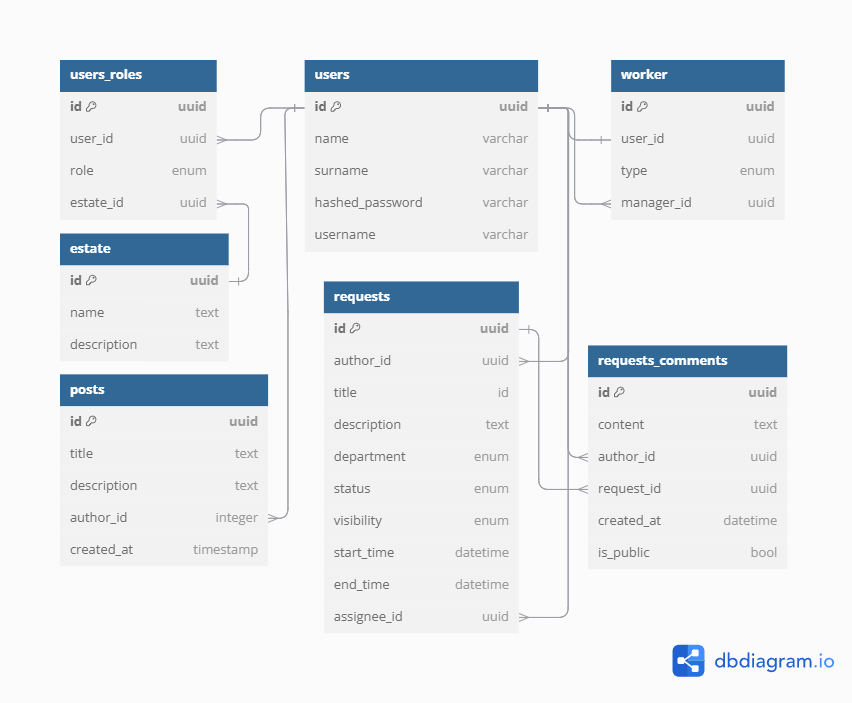
\includegraphics[width=1\linewidth]{img/ER_model.png}
    \caption{Model relacji}
    \label{fig:data model}
\end{figure}
Poniżej znajduje się reprezentacja relacji Requests (zgłoszenia) w kodzie Pythona z użyciem SQLAlchemy:
\begin{minted}{python}
    class Requests(Base):
        __tablename__ = "requests"

        id: Mapped[str] = mapped_column(primary_key=True, default=uuid.uuid4)
        author_id: Mapped[str] = mapped_column(ForeignKey(Users.id))
        title: Mapped[str] = mapped_column(String)
        description: Mapped[str] = mapped_column(String)
        department: Mapped[Enum] = mapped_column(Enum(Department),
                                                 nullable=True)
        status: Mapped[Enum] = mapped_column(Enum(Status), 
                                             default=Status.NEW)
        visibility: Mapped[Enum] = mapped_column(Enum(Visibility), 
                                                 default=Visibility.PRIVATE)
        start_time: Mapped[datetime.datetime] = mapped_column(DateTime)
        end_time: Mapped[datetime.datetime] = mapped_column(DateTime, 
                                                            nullable=True)
        assignee_id: Mapped[str] = mapped_column(ForeignKey(Users.id),
                                                 nullable=True)
\end{minted}

SQLAlchemy udostępnia wiele możliwości, takich jak reprezentowanie obiektów typem Enum zdefiniowanym w Pythonie, czy obiektami datetime. Daje to możliwość wygodniejszego użycia i analizowania działania bazy danych.

\subsubsection{Sposób korzystania z obiektów SQLAlchemy}
Jesteśmy w stanie zdefiniować funkcje używające konkretnych obiektów w celu np. wydobycia z nich danych, SQLAlchemy dostarcza możliwość nie pisania SQL-a tylko korzystania z zaimplementowanej biblioteki do budowania zapytań do bazy. Poniżej znajduje się przykład takiej funkcji zwracającej konkretne zgłoszenie:

\begin{minted}{python}
    def get_request(session, request_id: str, user_id: str) -> Requests | None:
        user_estate = get_user_estate_id(session, user_id)
        return (session.query(Requests)
                .select_from(Requests)
                .join(UsersRoles, 
                      UsersRoles.user_id == Requests.author_id)
                .filter(Requests.id == request_id,
                        UsersRoles.estate_id == user_estate)
                .first())
\end{minted}

\subsection{Implementacja użycia Elasticsearch'a}
\subsubsection{Struktura kodu}
\begin{itemize}
    \item queries.py - plik zawierający funkcje przeszukujące bazę
    \item utils.py - plik definiujący klienta
\end{itemize}
\subsubsection{Stworzenie klienta oraz wyszukanie informacji w bazie}
W celu połączenia z bazą Elasticsearch wykorzystana została biblioteka Elasticsearch, za pomocą której można utworzyć klienta oraz przeszukać bazę. Do przeszukiwania fragmentów tekstów w poszczególnych indeksach została wytworzona generyczna funkcja get\_ids\_for\_index\_containing. Oba te elementy można zaobserwować poniżej.
\begin{minted}{python}
    # utils.py file
    es_client = (
    Elasticsearch("http://elasticsearch-master.elk.svc.cluster.local:9200",
                  basic_auth="elastic",
                  verify_certs=False)
                )

    # queries.py file
    def get_index_for_id_containing(index: str, phrase: str) -> List[str]:
    """
    Get the id field of the hit containing the phrase in given index
    :param index: index name (eg. posts)
    :param phrase: phrase to look for
    :return: List of post ids
    """
        resp = es_client.search(index=index, 
                                query={"match": {"description": phrase}})
        return [x["_source"]["id"] for x in resp["hits"]["hits"]]
\end{minted}
\subsection{Konfiguracja pg\_sync}
Aby odpowiednie relacje były indeksowane w Elasticsearch należy dobrze skonfigurować pg\_sync. W ramach takiej konfiguracji poza plikiem przekazującym informacje o adresach i hasłach do baz, niezbędny jest również plik definiujący, które relacje powinny być indeksowane. Poniżej znajduje się fragment takiego pliku konfiguracyjnego wskazującego pg\_sync, aby indeksował trzy pola relacji posts: id, title oraz description.
\begin{minted}{json}
[
    {
        "database": "estate_management",
        "index": "posts",
        "nodes": {
            "table": "posts",
            "columns": [
                "id",
                "title",
                "description"
            ]
        }
    }
]
\end{minted}



\newpage
\section{Implementacja interfejsu użytkownika}
Interfejs użytkownika został zaimplementowany za pomocą języka typescript przy użyciu  biblioteki react pozwalającej na budowanie aplikacji internetowych. Użyto również framework-u css-owego tailwind umożliwiającego wygodne dostosowanie graficzne elementów strony. Do budowania strony użyto narzędzia Vite umożliwiającego zarówno budowanie wersji produkcyjnych jak i deweloperskich (odświeżających się w momencie zmiany kodu) w wygodny sposób.
\subsection{Podział kodu}
\begin{itemize}
    \item \textbf{assets} - pliki graficzne
    \item \textbf{components} - implementacje poszczególnych podstron
    \item \textbf{App.tsx} - główny komponent aplikacji zwracający Router aplikacji
    \item \textbf{index.css} - definicja użycia styli tailwind'a
    \item \textbf{main.tsx} - główny plik interfejsu zwracający główny komponent - App
    \item \textbf{router.tsx} - definicja routera aplikacji
    \item \textbf{types.tsx} - definicja typów użytych w aplikacji
\end{itemize}
\subsection{Implementacja komponentów}
W ramach interfejsu użytkownika zostały utworzone następujące podfoldery implementujące różne komponenty:
\begin{itemize}
    \item \textbf{estateAdmin} - komponenty odpowiedzialne za panel administratora
    \item \textbf{layout} - komponenty związane z całą stroną, np: Header
    \item \textbf{posts} - komponenty związane z ogłoszeniami
    \item \textbf{register}\_login - komponenty związane z logowaniem oraz rejestracją
    \item \textbf{requests} - komponenty związane ze zgłoszeniami
    \item \textbf{userPage} - strona użytkownika
    \item \textbf{utils} - wspólne części używane w wielu miejscach, np przycisk
\end{itemize}

Omówienie jednego z tych folderów umożliwi zrozumienie implementacji wszystkich, takim przykładowym folderów jest "requests", w którym znajdują się następujące pliki:
\begin{itemize}
    \item \textbf{comments} - komponenty związane z komentarzami pod danym zgłoszeniem
    \item \textbf{single} - komponenty związane z wyświetlaniem pojedynczego zgłoszenia
    \item \textbf{addRequest.tsx} - komponent zawierający formularz dodania pojedynczego zgłoszenia
    \item \textbf{fetches.ts} - plik zawierający wszystkie zapytania do API związane ze zgłoszeniami
    \item \textbf{RequestCard.tsx} - komponent wyświetlający pojedyncze zapytanie w formie kafelka
    \item \textbf{ViewRequests.tsx} - komponent wyświetlający wszystkie dostępne zapytania w formie kafelków
\end{itemize}
Większość komponentów składa się z podobnych elementów. Poniżej przedstawione są elementy komponentu requests/single/ViewRequest.
Pierwszym powtarzającym się elementem jest \textbf{zdefiniowanie zmiennych}
\begin{minted}{js}
export function ViewRequest() {
    const { requestId } = useParams<{ requestId: string }>();
    const [request, setRequest] = useState<RequestType>();
\end{minted}
Kolejnym jest \textbf{załadowanie danych}:
\begin{minted}{js}
useEffect(() => {
    getRequest(requestId!)
        .then((data) => setRequest(data))
        .catch((_) => {
            toastHelper.error("Wystąpił błąd :(. Spróbuj jeszcze raz");
        });
}, []);
\end{minted}
Załadowanie danych odbywa się za pomocą funkcji zdefiniowanej w pliku \textbf{request/fetches.ts}:
\begin{minted}{js}
export const getRequest = async (id: string): Promise<RequestType> => {
    const response = await fetch(`${API_ADDR}requests/${id}`, 
                                getSecureRequestOptions);
    if (!response.ok) {
        throw new Error("HTTP error " + response.status);
    }
    return await response.json();
}
\end{minted}
Typ używany powyżej \textbf{RequestType} zdefiniowany jest w pliku types.ts, który jest wspólny dla całej aplikacji. Poniżej znajduje się jego fragment definiujący RequestType:
\begin{minted}{js}
// Requests
export type RequestType = {
    id: string;
    author_id: string;
    title: string;
    description: string;
    department: string;
    status: string;
    start_time: string;
    end_time: string;
    assignee_id: string;
    visibility: string;
}
\end{minted}
Następnym elementem jest \textbf{zwrócenie odpowiednich komponentów}:
\begin{minted}{html}
return (
    <div>
        {isEmploye ? (
            <EditableView request={request} authorName={authorName} />
        ) : (
            <UserView request={request} authorName={authorName} />
        )}
        <div>
            <AllComments request_id={request.id} />
            <AddComment request_id={request.id} />
        </div>
    </div>
);
\end{minted}
Powyżej widzimy, że w zależności od typu użytkownika wyświetlane są poszczególne komponenty, zamieszczono przykład implementacji jednego z tych funkcji:
\begin{minted}{html}
function EditableView(props: { request: RequestType, authorName: string }) {
    return <div 
    className="p-12 grid grid-cols-1 md:grid-cols-2 gap-16 justify-center">
        <RequestInfo request={props.request} authorName={props.authorName}/>
        <RequestEdit request={props.request}/>
    </div>;
}
\end{minted}

Style pojedynczych komponentów często są poprawiane za pomocą przekazywania do zmiennej className odpowiednich atrybutów.

\newpage
\section{Dokładna implementacja wybranych funkcjonalności}
\subsection{Logowanie}
W implementacji logowania pomocnym był poradnik \cite{FastapiAuthLearn}.
Poniżej znajduje się diagram przepływu logowania, pokazują szczegółowo jego proces:

\begin{figure}[H]
    \centering
    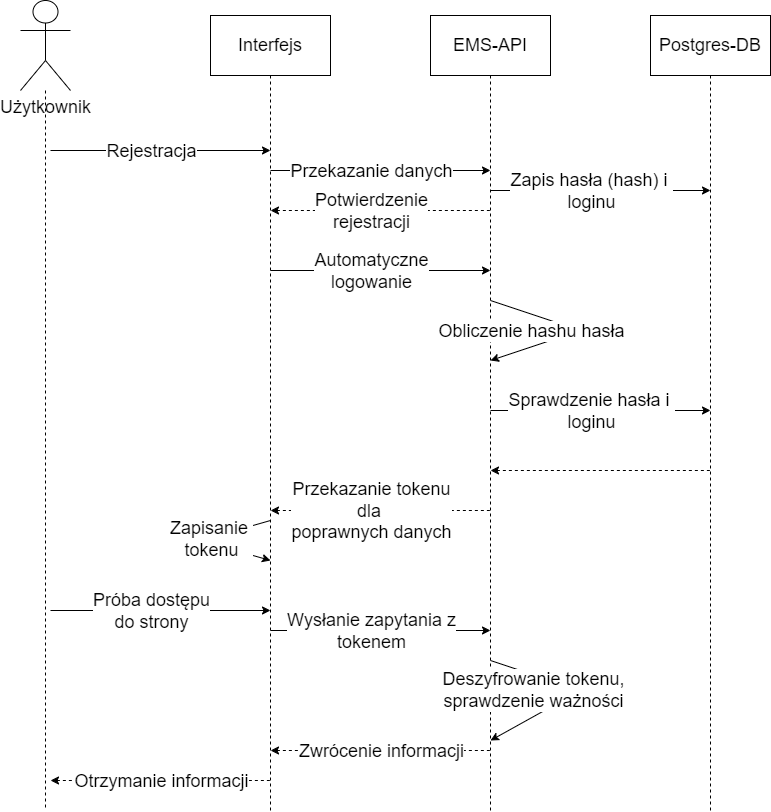
\includegraphics[width=0.75\linewidth]{img/sequence_login.png}
    \caption{Diagram przepływu logowania}
    \label{fig:seq-diag-login}
\end{figure}
Podczas logowania hasło użytkownika jest hash'owane oraz zapisywane w bazie za pomocą biblioteki passlib korzystającej z funkcji bcrypt. Podczas weryfikacji jest używana metoda verify.
\begin{minted}{python}
def verify_password(plain_password, hashed_password):
    return pwd_context.verify(plain_password, hashed_password)
\end{minted}

Gdy hasło użytkownika jest poprawne, tworzony jest token JWT. Token jest szyfrowany za pomocą klucza oraz algorytmu "HS256". Jest on następnie przekazywany klientowi oraz zapisany w local storage. Utworzenie tokenu o ważności 15 minut:
\begin{minted}{python}
def create_access_token(data: dict, expires_delta: timedelta | None = None):
    to_encode = data.copy()
    if expires_delta:
        expire = datetime.now(timezone.utc) + expires_delta
    else:
        expire = datetime.now(timezone.utc) + timedelta(minutes=15)
    to_encode.update({"exp": expire})
    encoded_jwt = jwt.encode(to_encode, SECRET_KEY, algorithm=ALGORITHM)
    return encoded_jwt
\end{minted}
Zapisanie go w local storage:
\begin{minted}{js}
    localStorage.setItem("accessToken", data.access_token);
\end{minted}
Przekazanie wraz z kolejnymi zapytaniami w nagłówku zapytania w celu weryfikacji:
\begin{minted}{js}
    method: "GET",
    headers: {
        "Content-Type": "application/json",
        "Authorization": `Bearer ${localStorage.getItem("accessToken")}`,
    }
\end{minted}
Przekazany token jest sprawdzany, na podstawie tokenu weryfikowany jest użytkownik oraz ważność tokenu.
\begin{minted}{python}
...
try:
    payload = jwt.decode(token, SECRET_KEY, algorithms=[ALGORITHM])
    username: str = payload.get("sub")
    if username is None:
        raise credentials_exception
    token_data = TokenData(username=username)
except InvalidTokenError:
    raise credentials_exception
...
\end{minted}
Po weryfikacji tokenu oraz użytkownika API zwraca konkretne informacje.